\documentclass[12pt]{beamer}
%\documentclass[20pt,handout]{beamer}
\usetheme{Darmstadt}
\usepackage{graphicx}
\usepackage[labelfont={bf,sf},font={small},labelsep=space]{caption}
\usepackage[ngerman]{babel}
\usepackage[T1]{fontenc}
\usepackage[utf8]{inputenc}
\usepackage{tikz}
\usepackage[shadow,colorinlistoftodos]{todonotes}
\setbeamertemplate{footline}[frame number]

\newcommand{\cc}[1]{\includegraphics[height=4mm]{img/#1.png}}
\usepackage{ifthen}
\newcommand{\license}[2][]{\\#2\ifthenelse{\equal{#1}{}}{}{\\\scriptsize\url{#1}}}
\usepackage{textcomp}

\setbeamercovered{transparent}

\pgfdeclareimage[height=.6cm]{c3d2logo}{./img/c3d2.pdf} 


\pgfdeclarelayer{foreground}
\pgfsetlayers{main,foreground}
\logo{\pgfputat{\pgfxy(-1,0)}{\pgfbox[center,base]{\pgfuseimage{c3d2logo}}}}


\title{Was mit Computern}
\author{\small Robert Wartenberg \& Johannes Lötzsch\\\large Chaos Computer Club Dresden}
\date{16.05.2018}

\begin{document}
\maketitle

\section{Einleitung}
\subsection{}

\begin{frame}
  \frametitle{Hacker}
  \begin{figure}
    
\includegraphics[height=0.7\textheight]{img/Glider.pdf}
  \end{figure}
\end{frame}

\begin{frame}
	\begin{center}
    	
\includegraphics[height=0.5\textheight]{img/cms-text.png}
    \end{center}
\end{frame}

\section{Einleitung}
	\subsection{}

\begin{frame}
	\frametitle{Chaos Computer Club}
	\begin{center}
		
\includegraphics[height=0.2\textheight]{img/chaosknoten.png}
	\end{center}	
	\begin{itemize}
		\item<1-> Verein wurde 1981 gegr"undet (\url{https://ccc.de})          
		\item<2-> Aktuell mehr als 6000 Mitglieder
		\item<3-> Betreibt u.a. "Offentlichkeitsarbeit und Politikberatung      
		\item<4-> Lokale Erfahrungsaustauschkreise (Erfas) und Chaostreffs
	\end{itemize}
\end{frame}

\begin{frame}
	\frametitle{Chaos Computer Club Dresden}
	\begin{center}
		
\includegraphics[height=0.1\textheight]{img/c3d2_logo.png}
	\end{center}
	\begin{itemize}
		\item<1-> Chaos Computer Club Dresden (\url{https://c3d2.de})          
		\item<2-> Datenspuren (\url{https://datenspuren.de})
		\item<3-> Radio und Podcasts (\url{https://c3d2.de/radio.html})
		\item<4-> Chaos macht Schule (\url{https://c3d2.de/schule.html})
	\end{itemize}
\end{frame}
  
\section{CmS}
\subsection{}
  
\begin{frame}
	\frametitle{Chaos macht Schule}
	\begin{itemize}
		\item<1-> seit ca. 2007
		\item<2-> Ehrenamtlich organisiert
		\item<3-> Bildung und Sensibilisierung
	\end{itemize}
\end{frame}
  
\begin{frame}
	\frametitle{Zielgruppe}
	\begin{itemize}
		\item<1-> Schüler*innen
		\item<2-> Lehrer*innen
		\item<3-> Eltern 
	\end{itemize}
\end{frame}
  
\begin{frame}
	\frametitle{Inhalte}
	\begin{itemize}
		\item<1-> Datenschutz gegen Überwachung
			\only<1>{
				\begin{center}
				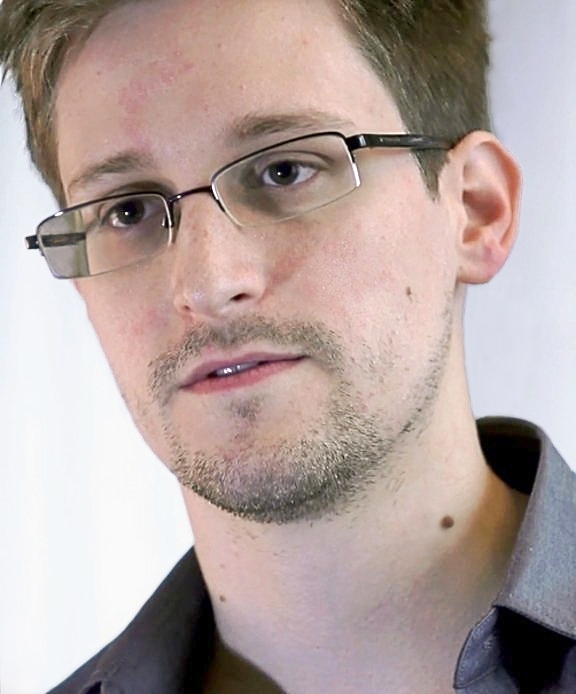
\includegraphics[height=0.7\textheight]{img/snowden.jpg}
				\end{center}
			}
			\only<2>{
				\begin{center}
				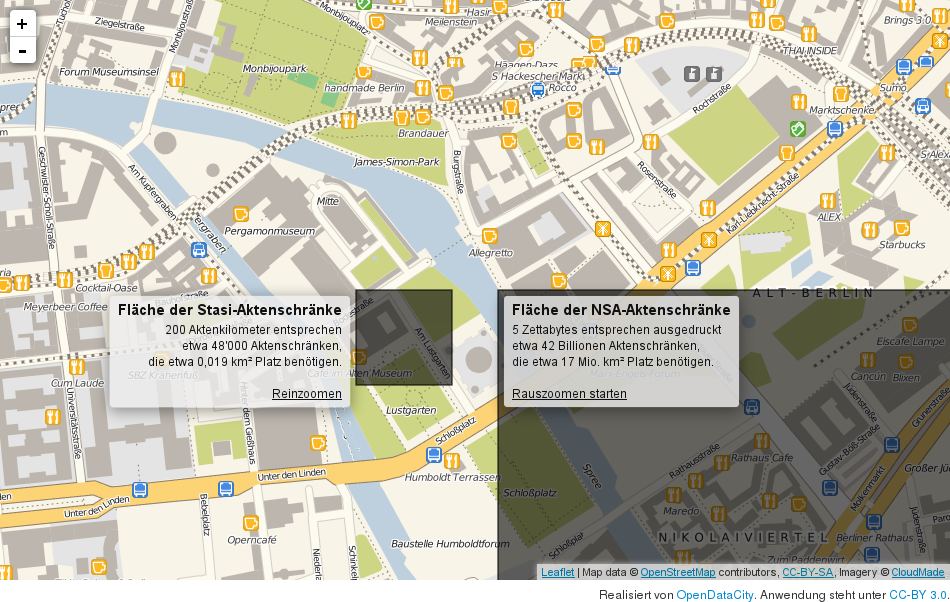
\includegraphics[height=0.7\textheight]{img/akten1.png}
				\end{center}
			}
			\only<3>{
				\begin{center}
				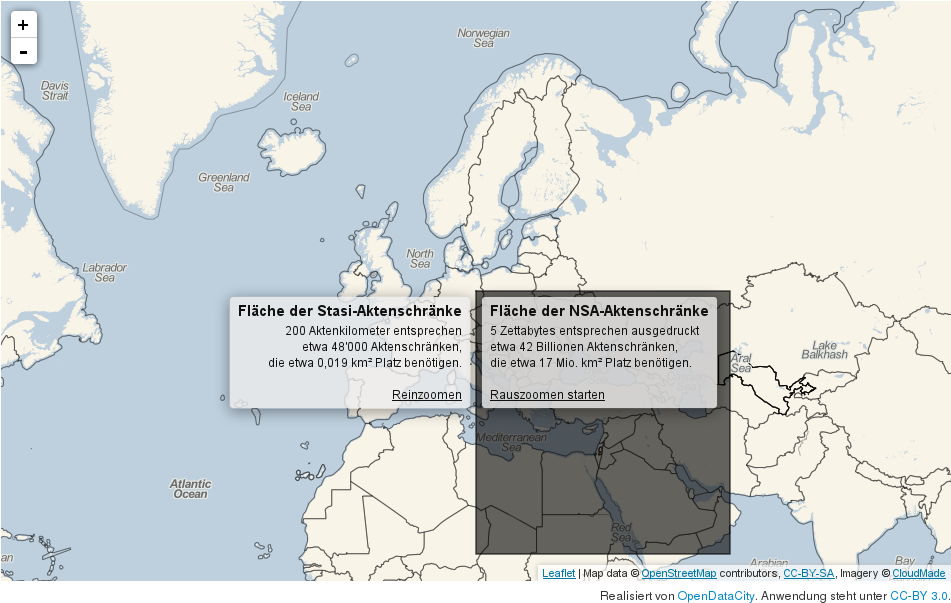
\includegraphics[height=0.7\textheight]{img/akten2.png}
				\end{center}
			}
			\only<4>{
				\begin{center}
				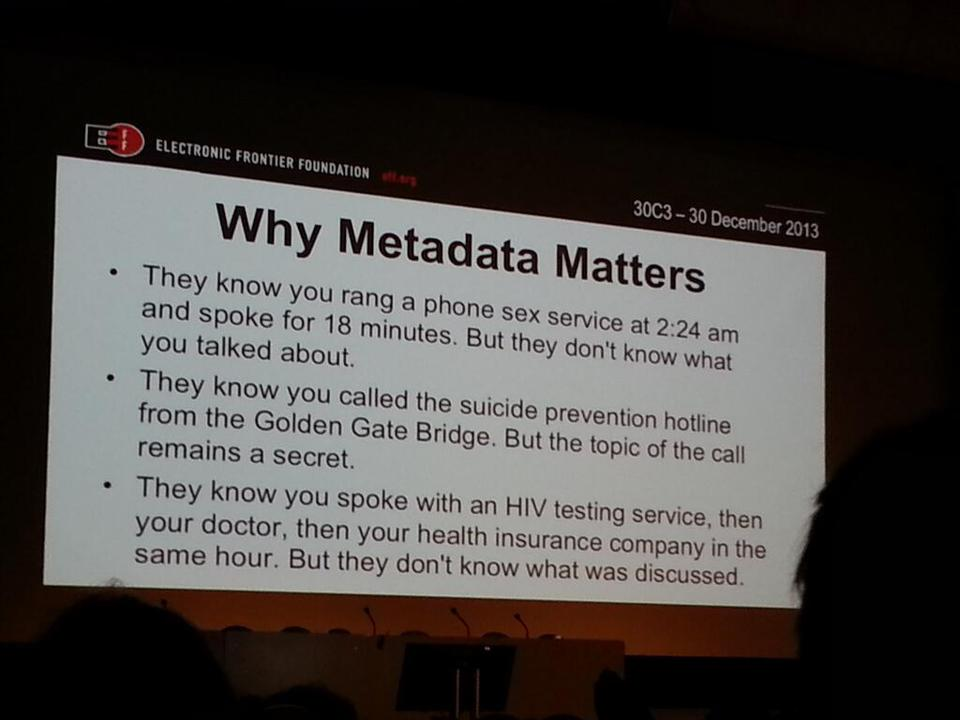
\includegraphics[height=0.7\textheight]{img/metadata-matters.jpg}
				\end{center}
			}
			\only<5>{
				\begin{center}
				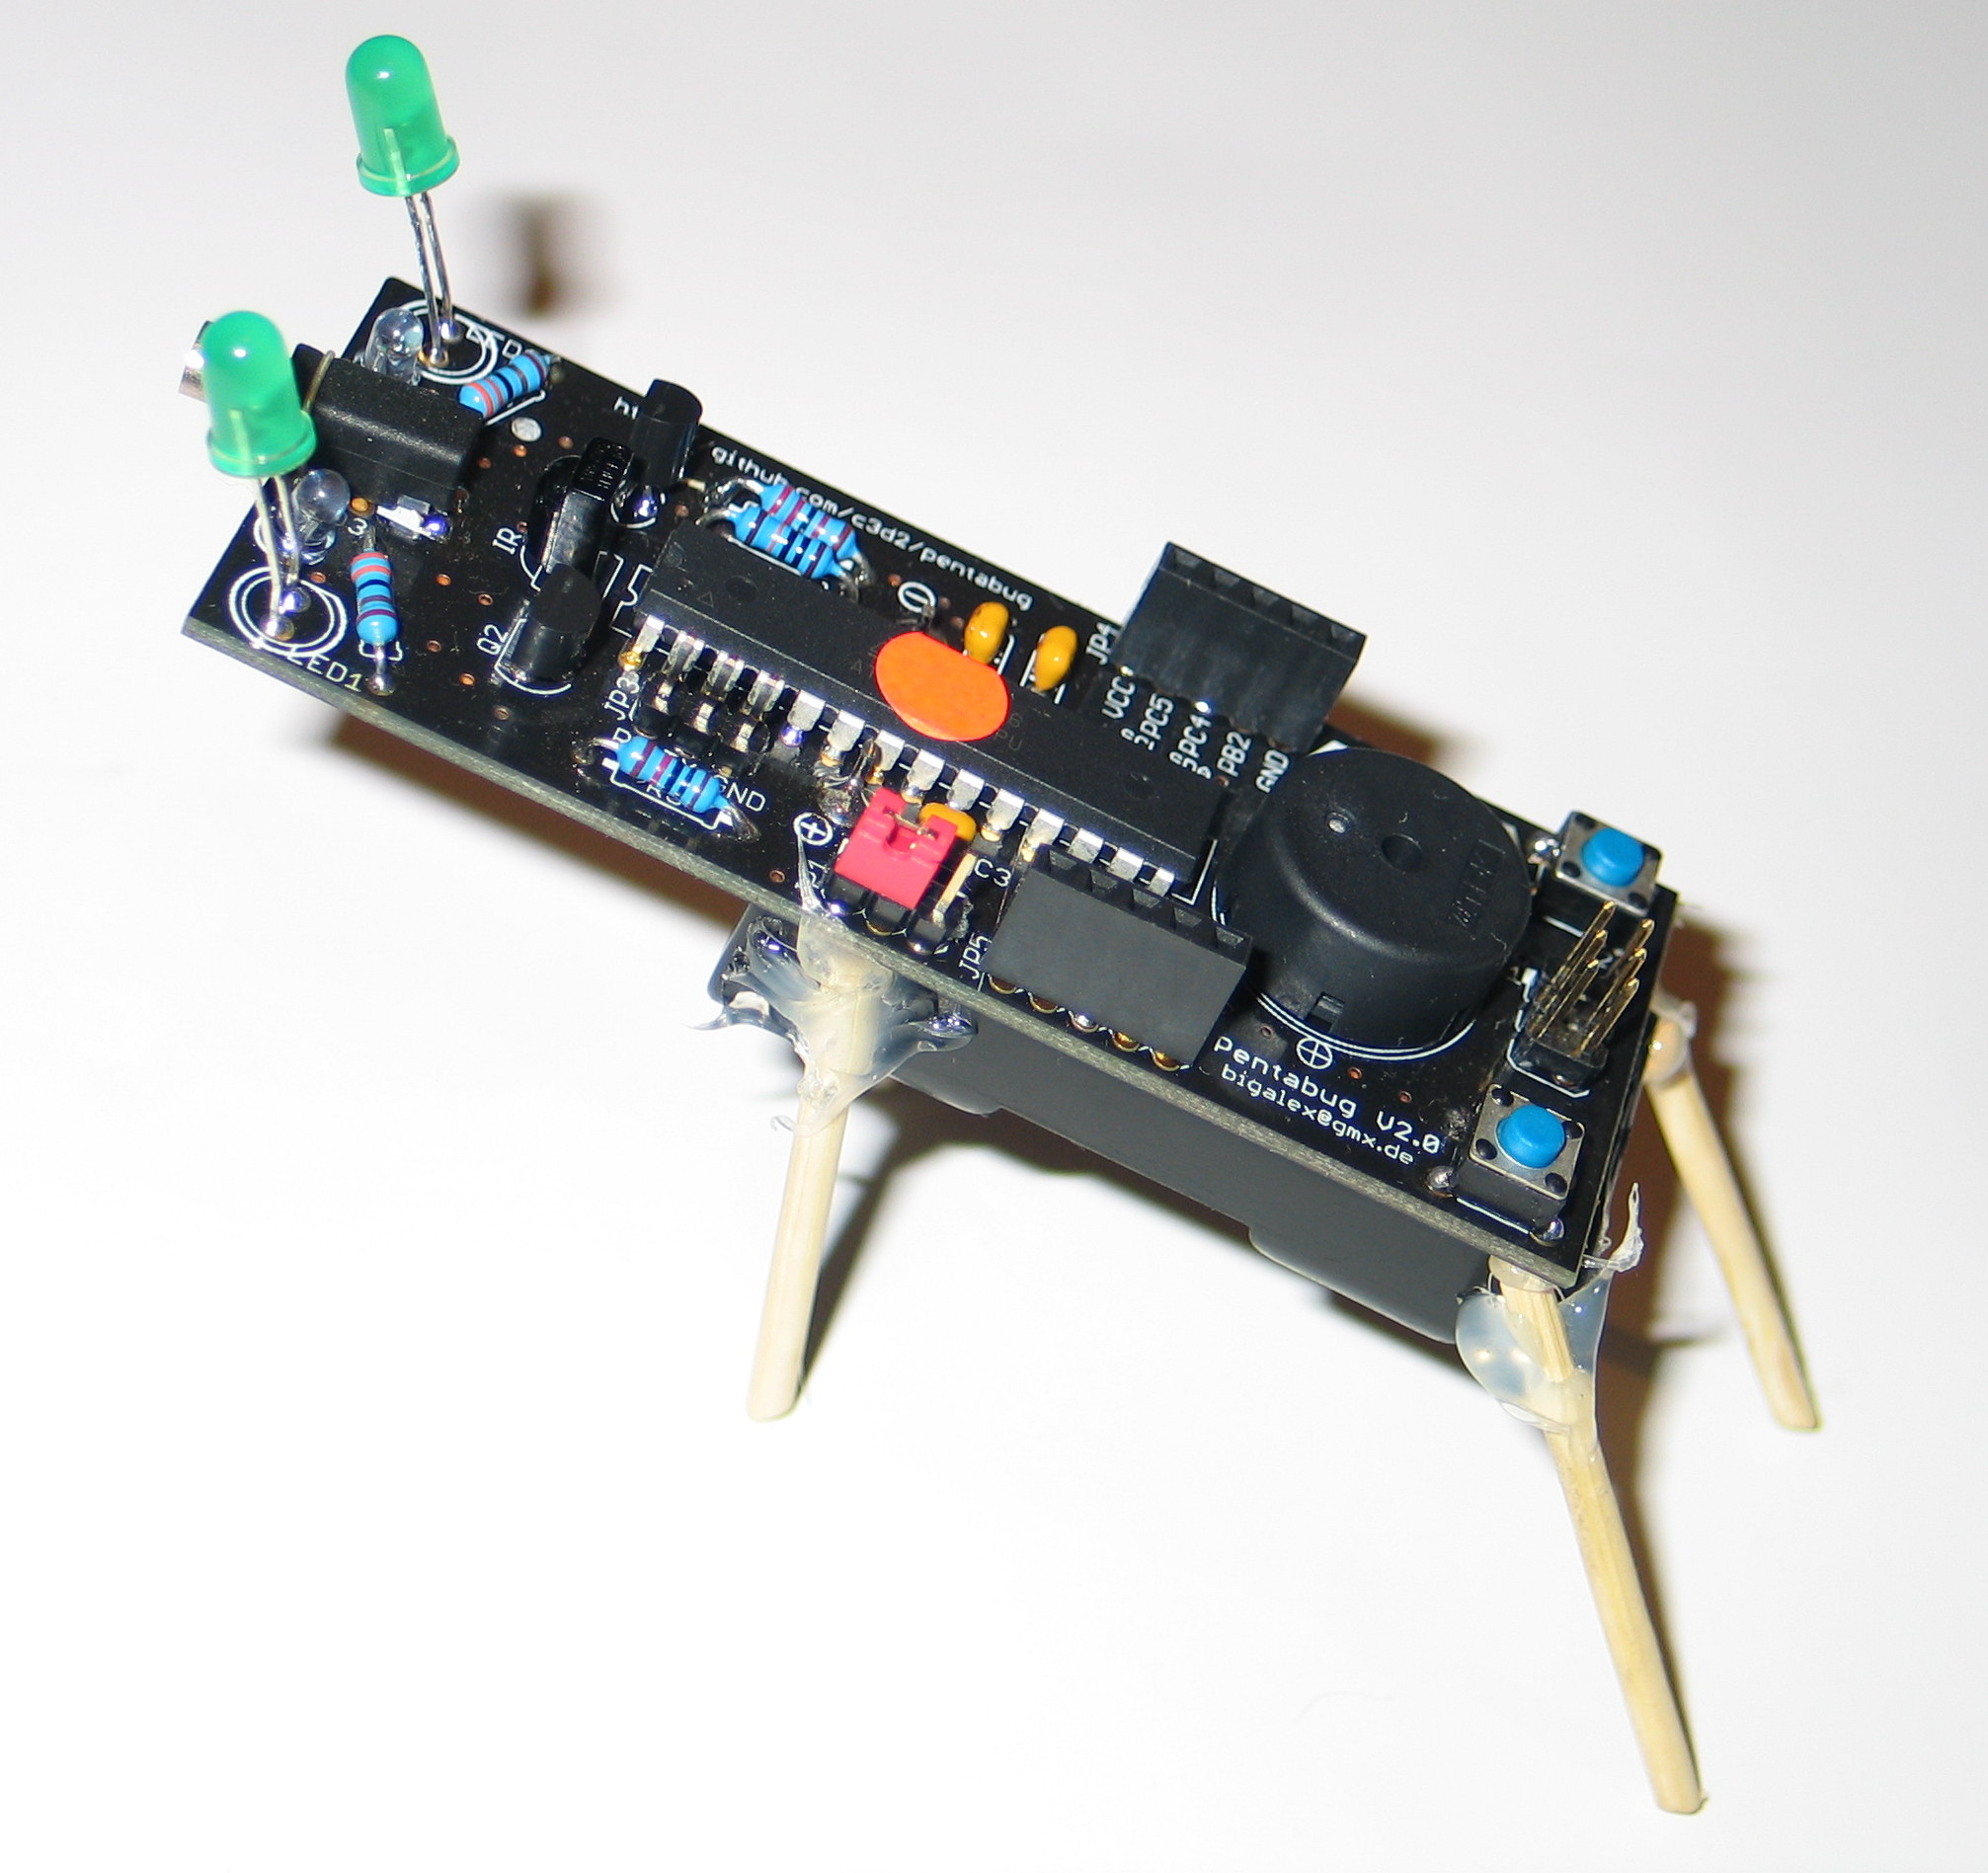
\includegraphics[height=0.5\textheight]{img/pentabug.jpg}
				\end{center}
			}
		\item<6-> Sensibilisierung für freie Software
		\item<7-> Bildung über verschiedene Dienste / Software
		\item<8-> Workshops
	\end{itemize}
\end{frame}

\begin{frame}
  \frametitle{Themen}
  \begin{figure}
    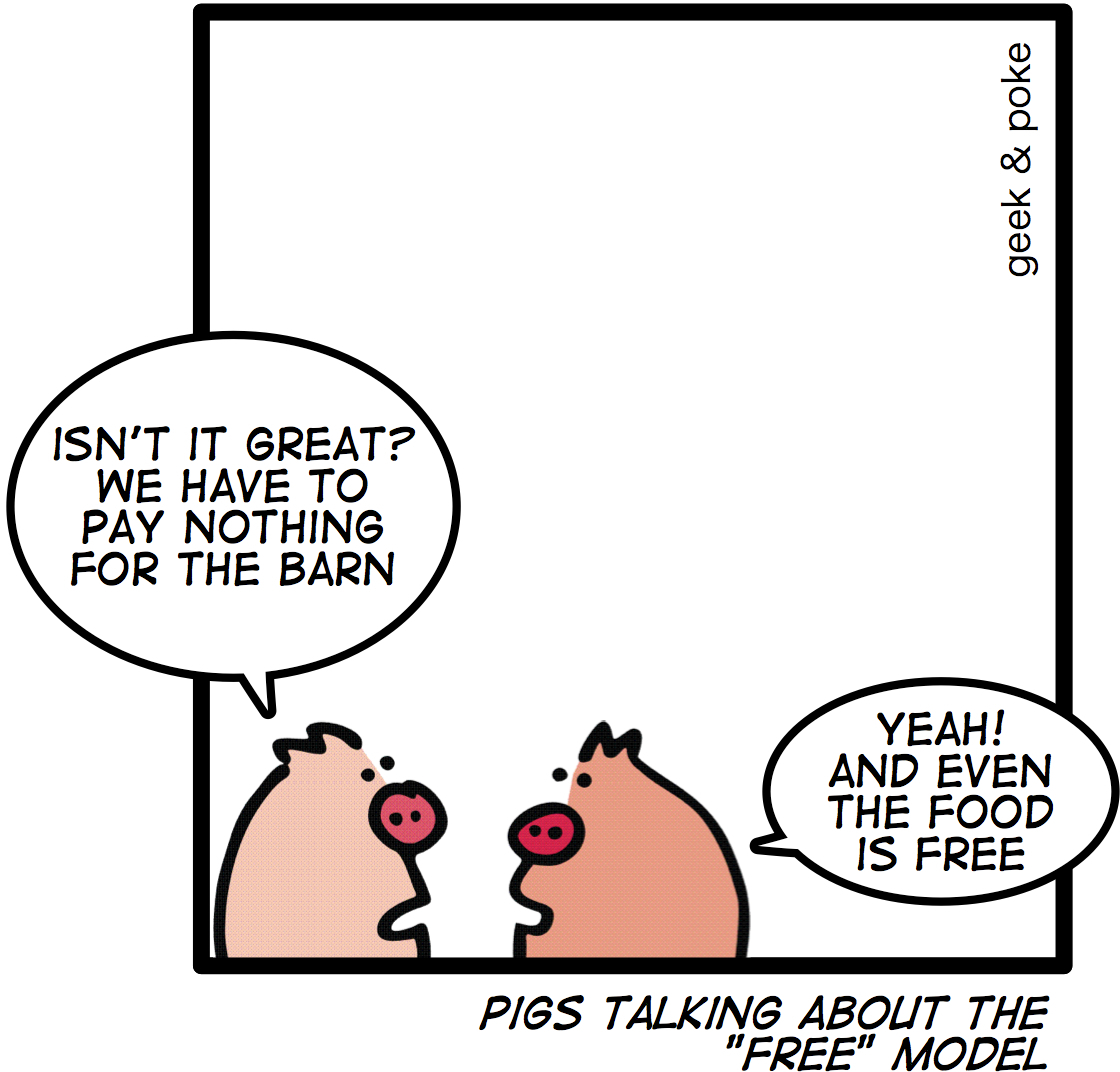
\includegraphics[height=0.7\textheight]{img/business_pigs.jpg}
  \end{figure}
\end{frame}


\section{Internet}
\subsection{}

\begin{frame}
	\frametitle{Was ist es für ...}
	\begin{itemize}
		\item<1-> Kinder?
		\begin{center}
			\only<2>{
				
\includegraphics[height=0.7\textheight]{img//magic_internet.jpg}
			}
		\end{center}
		\item<3-> Jugendliche?
		\begin{center}
			\only<4>{
				
\includegraphics[height=0.7\textheight]{img//social_networks.jpg}
			}
		\end{center}
		\item<5-> Senioren
		\begin{center}
			\only<6>{
				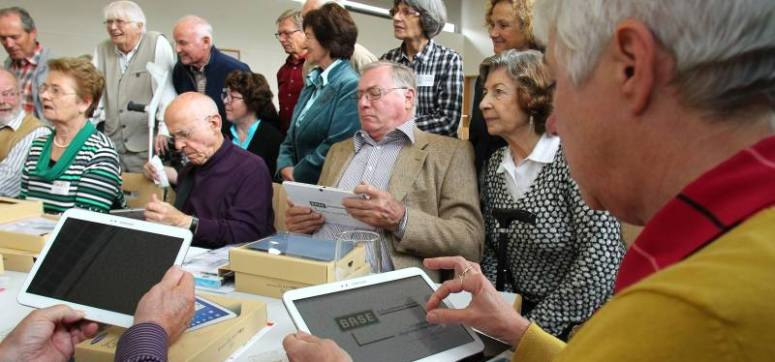
\includegraphics[height=0.5\textheight]{img//senior.jpg}
			}
		\end{center}
		\item<7-> euch?
		\begin{center}
			\only<7>{
				
\includegraphics[height=0.4\textheight]{img//frage.jpg}
			}
		\end{center}
	\end{itemize}
\end{frame}
  
\begin{frame}
	\frametitle{Internet}
	\begin{center}
		\only<1>{
			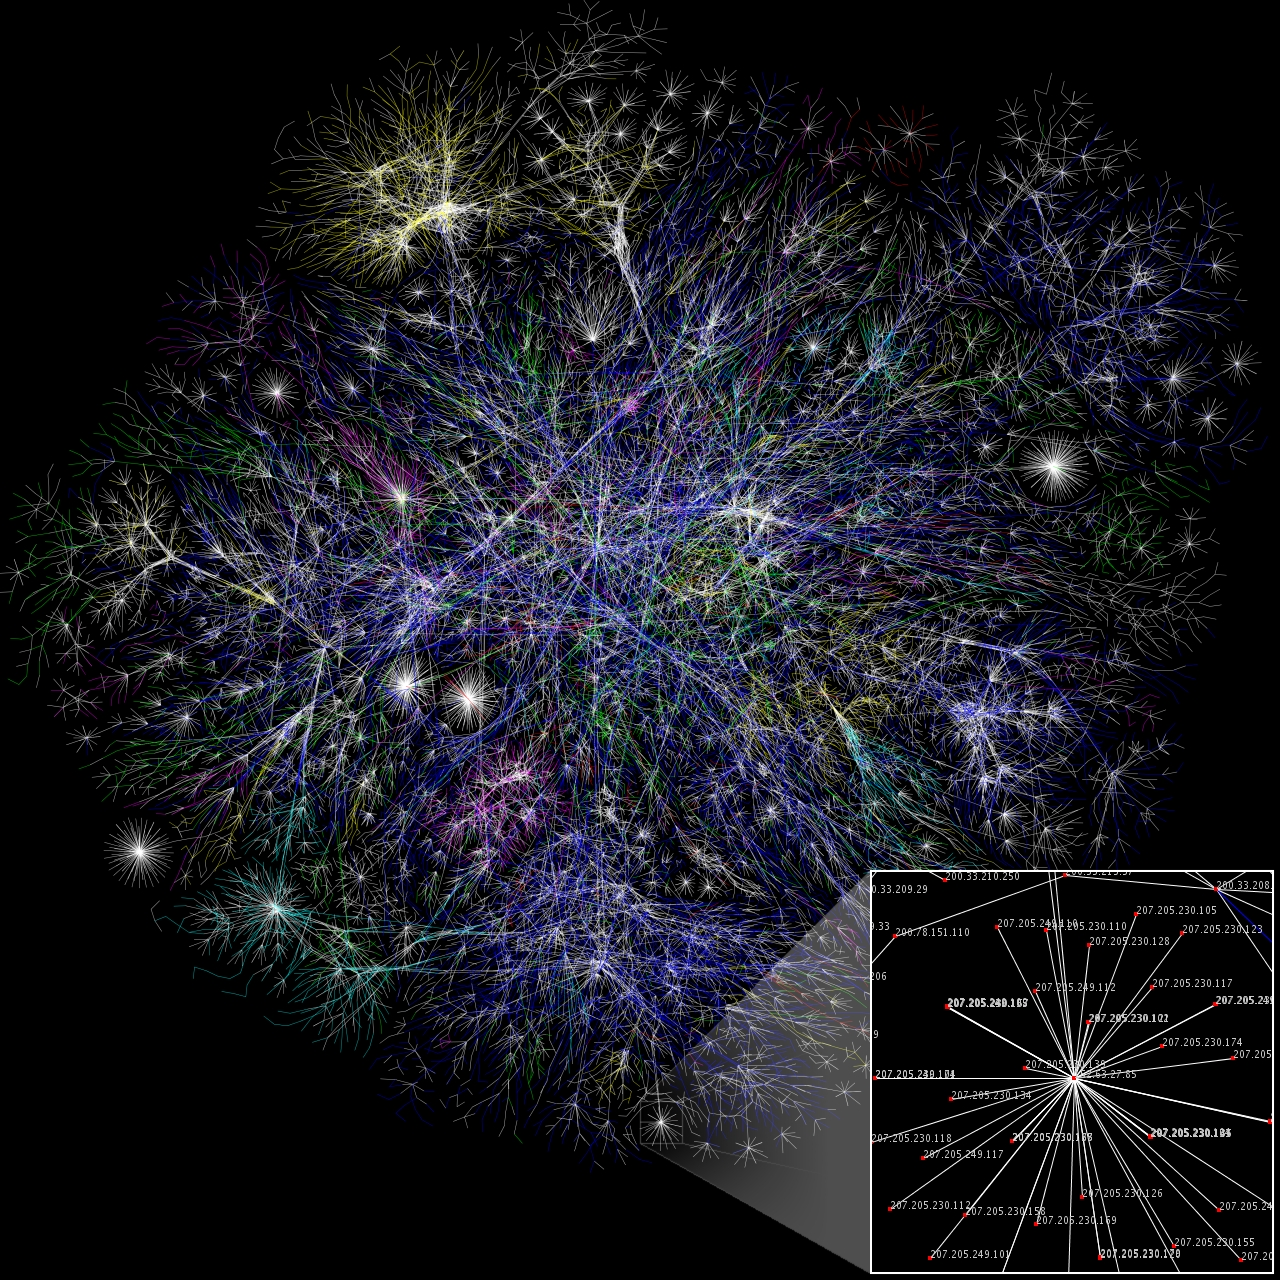
\includegraphics[height=0.7\textheight]{img//internet_0.jpg}
		}
		\only<2>{
			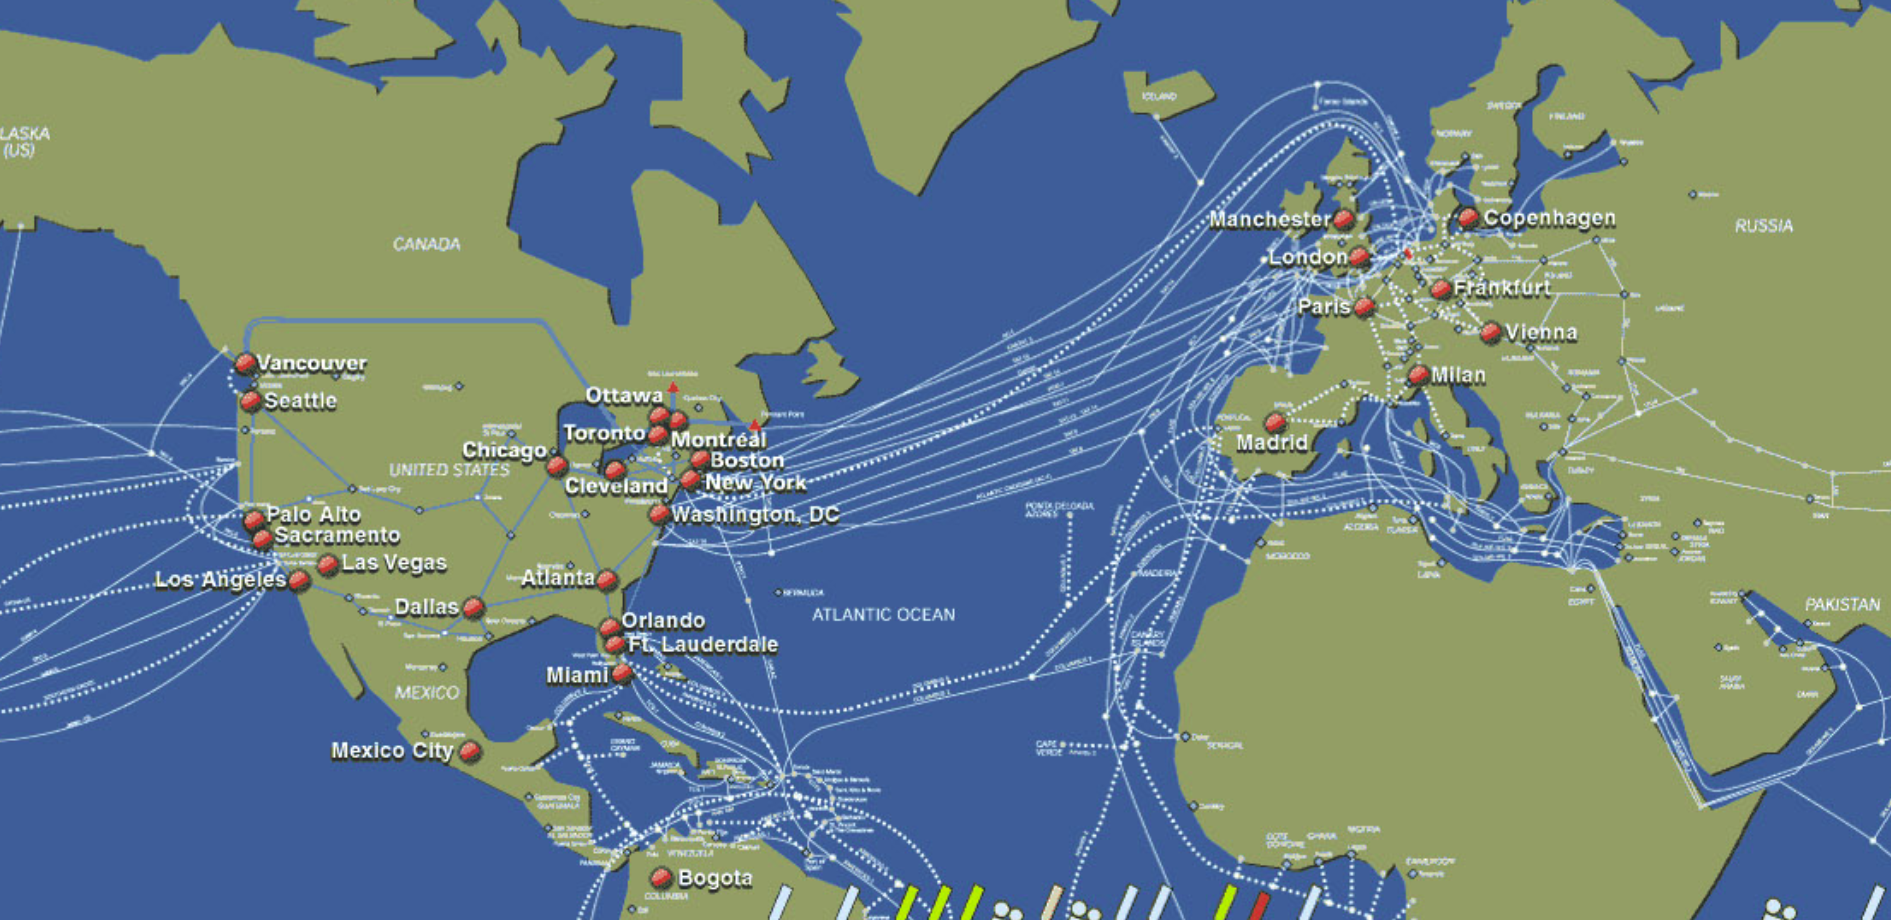
\includegraphics[height=0.6\textheight]{img//internet_1.png}
		}
		\only<3>{
			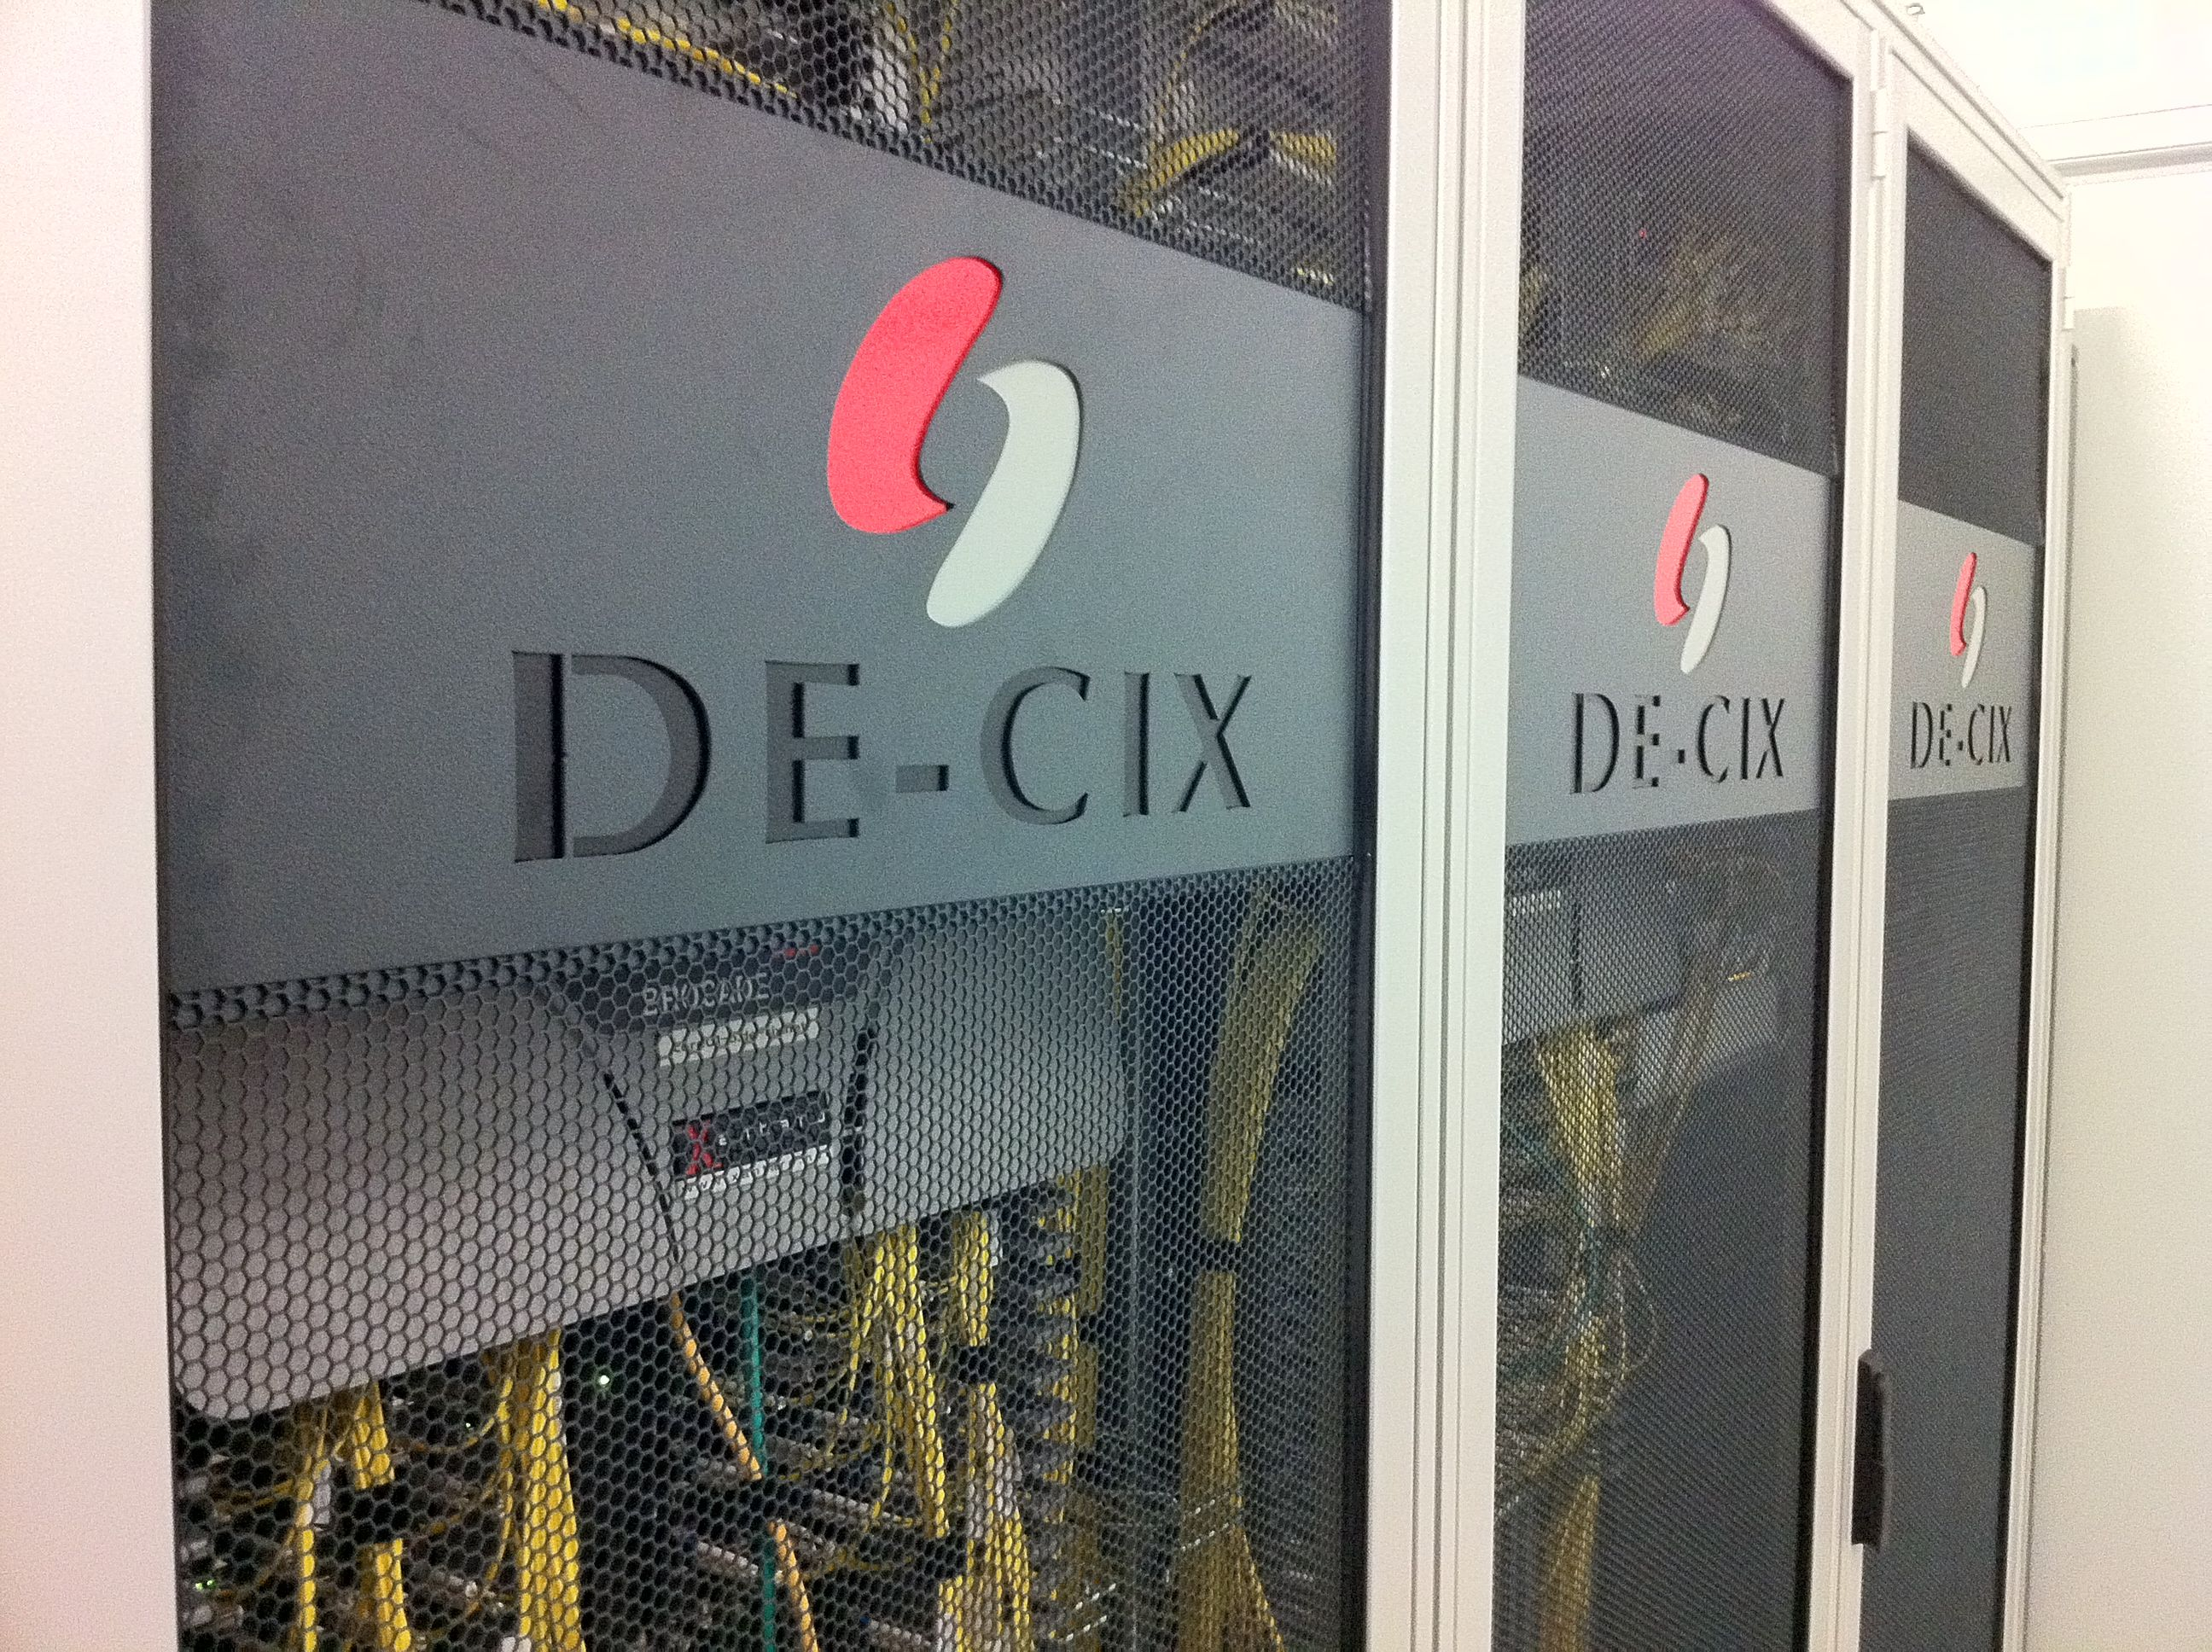
\includegraphics[height=0.6\textheight]{img//internet_2.jpg}
		}
	\end{center}
\end{frame}

\begin{frame}
	\frametitle{Fazit Internet}
	\begin{itemize}
		\item<1-> dezentral
		\item<2-> senden und empfangen
    \item<3-> neutral
	\end{itemize}
\end{frame}

\begin{frame}
	\frametitle{Fazit Internet}
  \begin{itemize}
    \item<1-> Netzwerkeffekte 
    \only<1>{
      \begin{center}
      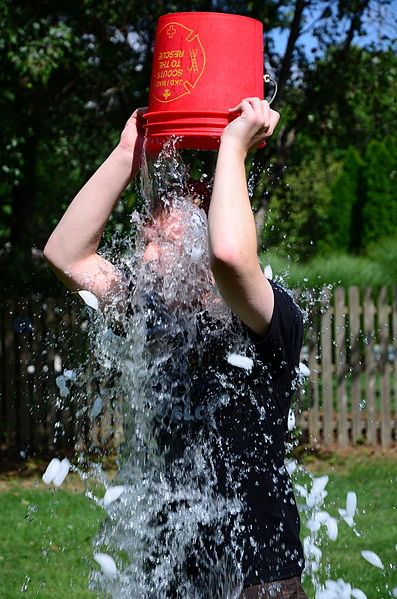
\includegraphics[height=0.5\textheight]{img//Doing_the_ALS_Ice_Bucket_Challenge_wiikipedia.jpg}
      \end{center}
    }
    \item<2-> Echokammern
    \item<3-> digitaler Tribalismus
    \only<3>{
      \begin{minipage}{\linewidth}
          \centering
          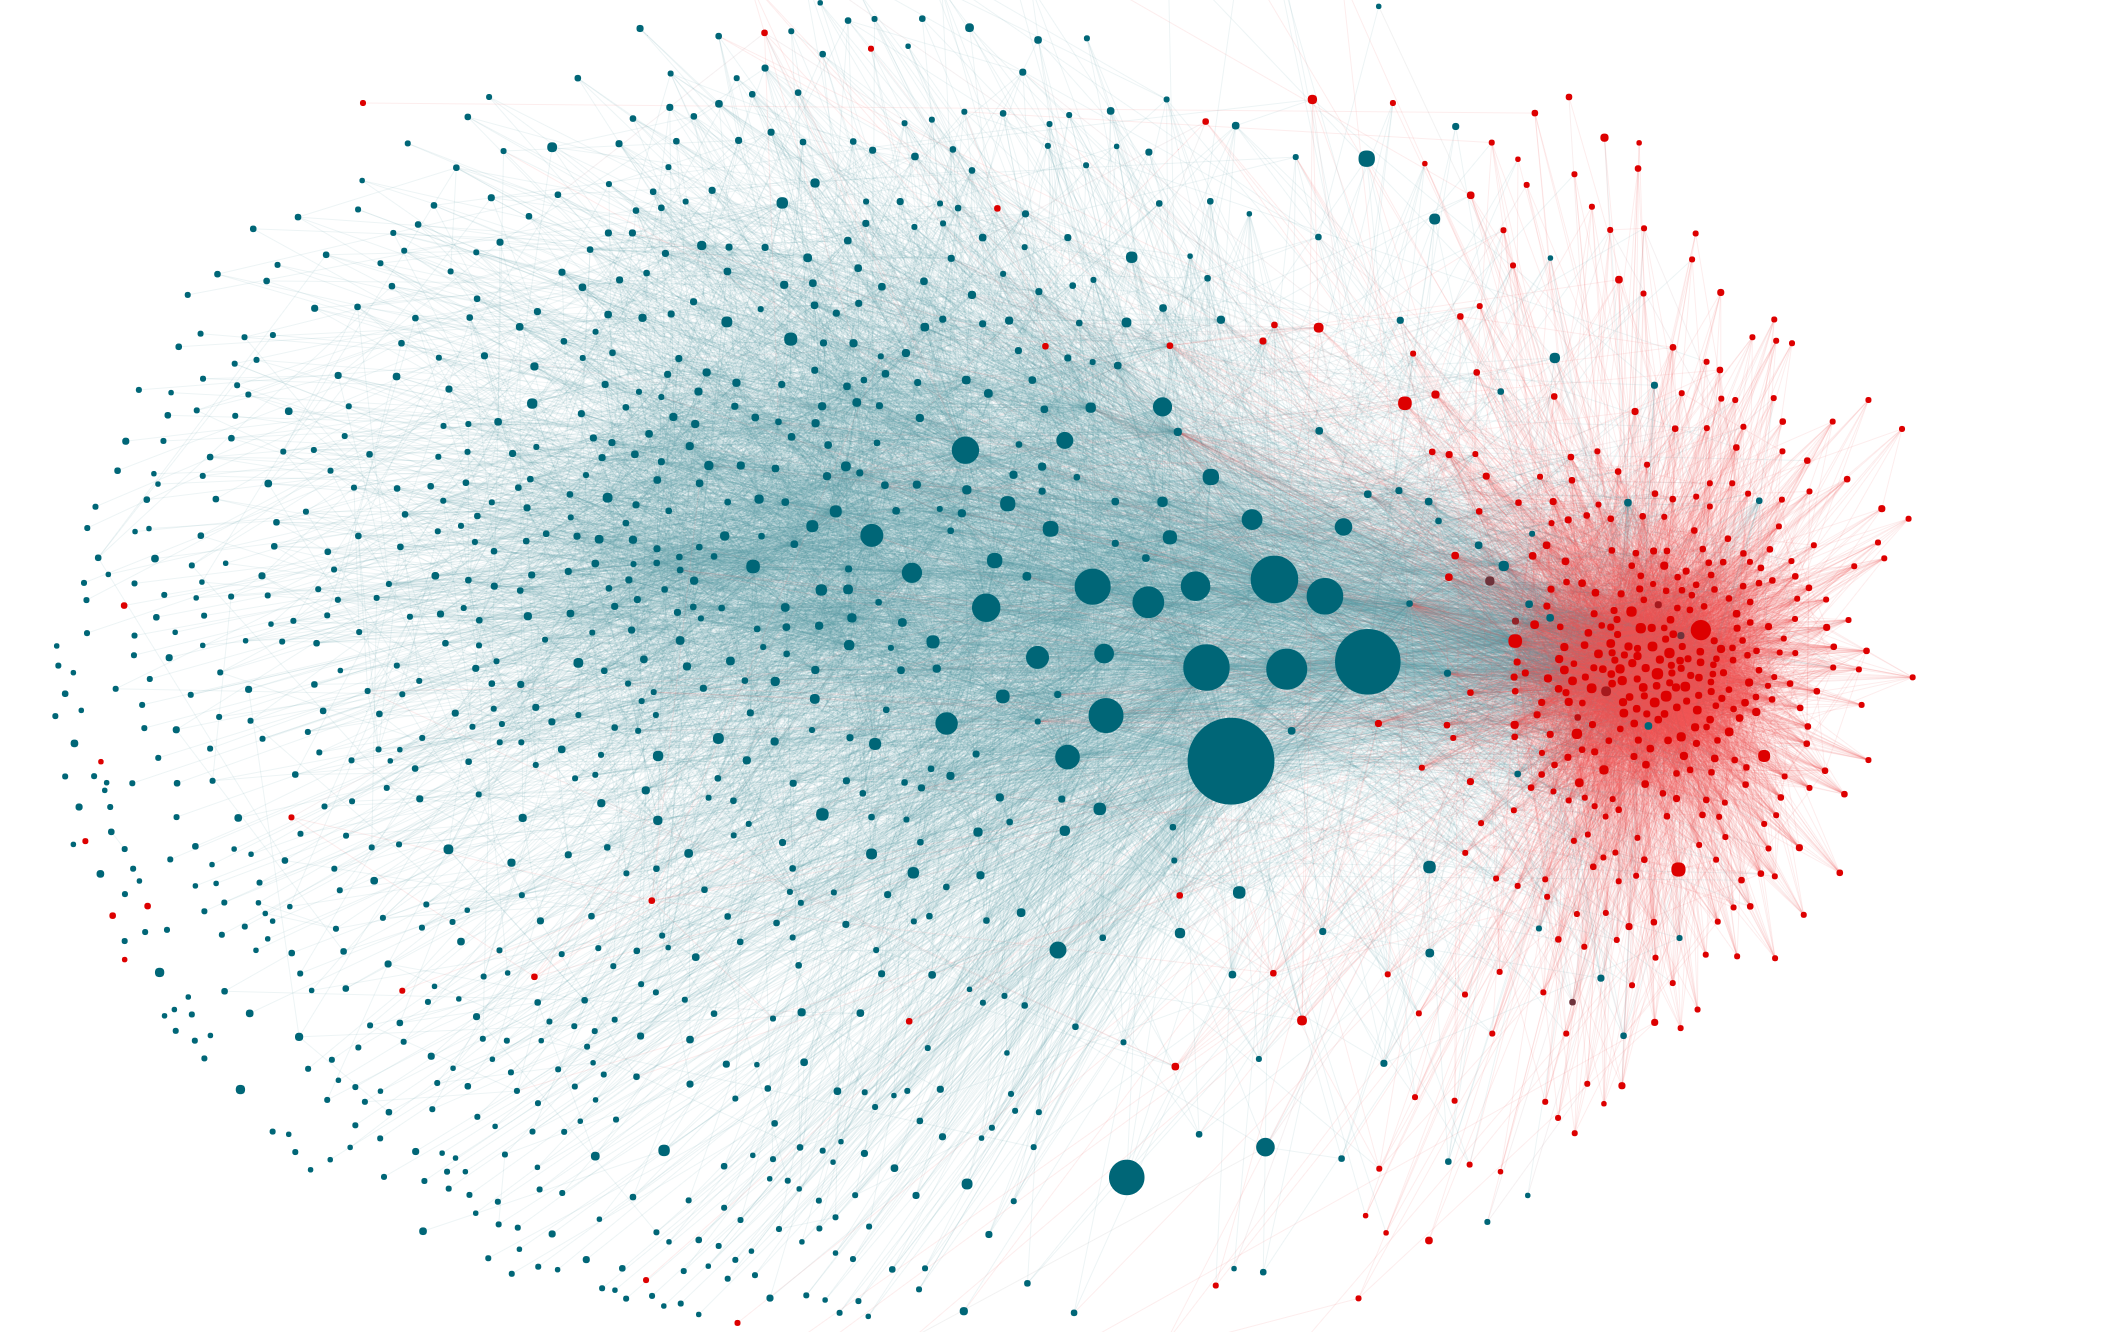
\includegraphics[height=0.5\textheight]{img//digitaler_Tribalismus_Terrorwarnstufe_Schweden.png}
      \end{minipage}
    }      
  \end{itemize}		
\end{frame}

\section{Im Unterricht}
\subsection{}

\begin{frame}
	\frametitle{Beispiele}
	\begin{itemize}
		\item<1-> Deutsch
			\begin{itemize}
				\item<1-> eigene Wikis lesen/schreiben
				\item<2-> Fremdsprachler im Netz lehren
			\end{itemize}
		\item<2-> Mathe
			\begin{itemize}
				\item<2-> Verschlüselung
				\item<1-> Lernvideos und interaktive Plattformen, Spiele
				\item<2-> Binäres rechnen
				\item<2-> "binär -> bool -> Matrixisplay"
				\item<2-> Tafelbild Matrixdisplay
			\end{itemize}
		\item<2-> Biologie
			\begin{itemize}
				\item<1-> Zellolärere Automaten
				\item<2-> KI Beispile (https://js.tensorflow.org/)
				\item<2-> Fortbewegungsarten von Robotern studieren an Hand der Natur
			\end{itemize}
		\item<2-> Geschichte
			\begin{itemize}
				\item<1-> http://histropedia.com/timeline
				\item<2-> Ahnenforschungswebseiten
				\item<2-> Regionalbezug Zuse / Hoyerswerde Museeum
				\item<2-> "Aus der Geschichte für die Zukunft lernen"
			\end{itemize}
		\item<2-> Sport
			\begin{itemize}
				\item<1-> Quantified Yourself Bewegung
				\item<2-> Cyborgs
			\end{itemize}
		\item<2-> Physik
			\begin{itemize}
				\item<1-> 
				\item<2-> 
			\end{itemize}
	\end{itemize}
\end{frame}


\section{Zukunft}
  \subsection{}
  
\begin{frame}
	\frametitle{Ein Blick in die Zukunft der Wirtschaft}
	\begin{itemize}
		\item<4-> Digitalisierung / Automatisierung
    \item<1-> Überwachung -> Daten!
		\item<2-> Neuronale Netze
		\item<3-> DATEN!!!		
	\end{itemize}
\end{frame}

\begin{frame}
	\frametitle{Ein Blick darüber hinaus..}
	\begin{itemize}
		\item<1-> Wissen und Vernetzung
		\item<2-> Miniaturisieung
		\item<3-> freie Infrastrukturen
	\end{itemize}
\end{frame}


\begin{frame}
	\frametitle{Schlussworte}
	\begin{itemize}
		\item<1-> Zukunft?
		\item<2-> Lernen, Lernen, Lernen
		\item<3->  
	\end{itemize}
\end{frame}

\section{Ende}
	\subsection{}

\begin{frame}
	\frametitle{Danksagung}
	\begin{center}
		\textbf{Ein Dank geht an:}
		\begin{itemize}
			\item<1-> die Fakultät für die Einladung
			\item<2-> an euch für das Interesse
			\item<2-> nicht an Apple oder Microsoft! ;-)
		\end{itemize}
	\end{center}
\end{frame}
  
\begin{frame}
	\frametitle{Ende}
	\begin{center}
		\textbf{Danke für eure Aufmerksamkeit!} \\
		\textbf{Kontakt: schule@c3d2.de} \\
		\textbf{Fragen?} 
	\end{center}
	\begin{itemize}
		\item<1-> https://c3d2.de/
		\item<2-> https://c3d2.de/schule.html
		\item<4-> https://lists.c3d2.de/  
	\end{itemize}
\end{frame}

\begin{frame}
	\begin{center}
    	
\includegraphics[height=0.5\textheight]{img//cms-text.png}
    \end{center}
\end{frame}

\end{document}
